\documentclass[11pt]{article} % use larger type; default would be 10pt


%%% PAGE DIMENSIONS
\usepackage[top=1in, bottom=1in, left=1in, right=1in]{geometry} % to change the page dimensions
 
%%% PACKAGES
\usepackage{graphicx} % support the \includegraphics command and options
\usepackage{amsfonts}
\usepackage{amsmath}
\usepackage{tikz}
\usepackage{graphicx}

 
%%% The "real" document content comes below...

\title{CS 134 \\ \emph{Problem Set 3}}
\author{Xiner Zhou}
\date{\today} % Activate to display a given date or no date (if empty),
        

\begin{document}
 
\maketitle

  
\paragraph{1. Non-Preferential Attachment (20 points).} 

\begin{itemize}
	\item[\textbf{a.}] \textbf{(8 points)}  

Let $Z_k(t)$  be the random variable denoting node $i_k$ receives an edge at time t, where $k \in \{1, \dots, t-1\}$.  For $t>k$:
$$Z_k(k+1)=\frac{1}{k}$$
$$Z_k(k+2)=\frac{1}{k+1}$$
$$ \dots $$
$$Z_k(t)=\frac{1}{t-1}$$

Let $X_k(t)$  be the random variable denoting the in-degree of node $i_k$ at time t, where $k \in \{1, \dots, t-1\}$. Then, 
$$X_k(t):=\sum_{T=k+1}^t Z_k(T)$$
$$=\frac{1}{k}+\frac{1}{k+1}+\dots+\frac{1}{t-1}$$
$$=\sum_{i=1}^{t-1} \frac{1}{i} - \sum_{i=1}^{k-1} \frac{1}{i}$$
$$\approx log(t-1) - log(k-1) $$
$$=log(\frac{t-1}{k-1})$$

	
	
	\item[\textbf{b.}] \textbf{(8 points)} 
\begin{eqnarray}
X_k(t)= log (\frac{t-1}{k-1}) \geq d \\
\Rightarrow \frac{t-1}{k-1}  \geq e^d \\
\Rightarrow k  \leq \frac{t-1}{e^d}+1
\end{eqnarray}

Therefore, at time step t, the fraction of nodes that have expected in-degree at least d is: 
$$ \frac{\frac{t-1}{e^d}+1}{t}=\Theta(\frac{1}{e^d})=\Theta(e^{-d})$$ 

	\item[\textbf{c.}] \textbf{(4 points)}

No, I don't expect the graphs genreated using this method to have a power-law degree distribution. 

If we believe the rich-get-richer model or the preferential-attachment model explains the underlying mechanism of the observed "popularity" in network follows a power-law distribution, 	then, we have proven in class that the number of in-degree will be distributed approximated as a power-law $c k^{-\alpha}$, with $c = \frac{1-p}{p} and \alpha = \frac{1}{1-p}$ where $p$ is the probability of a node choosing existing a node uniformly at random from all previous nodes. Power law arises from the feedback introduced by correlated decisions across population. In the rich-get-richer model, this dependency or correlation is represented by $1-p$: as $p$ gets smaller, $1-p$ gets larger, dependency is stronger, that is, copying becomes more frequent, making it more likely to see extreme popular items in the network, this is when the power law is stronger.
 
In this case, we have $1-p =0$, basically there is no copying mechanism or no preferential attachment, there is an absence of fundamental mechanism that generates power-law phenomena.


\end{itemize}









\paragraph{2. Power Laws in Classrooms [Easley and Kleinberg, 18.8 Q3] (10 points).}    


I expect that Harvard classes to be more closely follow a power-law distribution as a function of $k$.  

Power-law distribution is widespread in cases where the quantity being measured can be viewed as a type of popularity (this case certainly is!). And we use the rich-get-richer model or preferential-attachment model to explain the mechanism why the power law arises. The essence of the rich-get-richer model is the copying mechanism, which basically saying: every node in the network has a probability of $p$ not to copy the decision of a random previous people; and has a probability of $1-p$ to copy previous people's choices,and end up linking to some node $i$ with the probability proportional to the number of links $i$ already has. Because the probability of node $i$ increases popularity is directly proportional to the its current popularity. This so-called preferential-attachment phenomena is the basic mechanism that gives rise to power-law distribution, and is stronger when $1-p$ is larger, that is, when people tend to copy other's behavior more often.  

Harvard student group is a much smaller, more inter-connected social network, compared to the third-grade school students spread out through New York state, where kids in different districts may not even know each other. Beside the connectivity structure of the two networks, Harvard students are more likely to seek class information and based their decision on information through peers. College classes is more challenging at Harvardl, and which classes to take partial decide the college experience, as well as future career. Therefore, Harvard college students have more incentives to share and seek class information, and they have more resources to help them do so, like reviews and ratings from previous takers.  

Therefore, the likelihood of preferential attachment is much higher for Harvard classes, and thus is more likely to follow a power-law distribution.








\paragraph{3. It's a Power-Law Story (15 points).}

First, calculate the value of $c$: 
$$\sum_{k=1}^{485,165,195} P(X=k) =c \sum_{k=1}^{485,165,195} \frac{1}{k^2} =1 $$
$$\Rightarrow c=\frac{1}{\sum_{k=1}^{485,165,195} \frac{1}{k^2}} \approx \frac{6}{\pi^2}$$
 

Second, calculate the expected rerevue from selling the single:
$$E(Revenu) =\sum_{k=1}^{485,165,195} P(X=k) \times k  $$
$$ =\sum_{k=1}^{485,165,195} c \frac{1}{k^2} \times k $$
$$ =c \sum_{k=1}^{485,165,195} \frac{1}{k}$$
$$ = \frac{6}{\pi^2} log(485,165,195)$$
 $$= \frac{6}{\pi^2} \times 20 $$
$$ =12.15854 $$

Finally, calculate the expected profit: 
$$ E(Profit) = E(Revenu) - 100 = -87.84146 <  0 $$

Therefore, people should not purchase the right, if trying to make a positive profit.








\paragraph{4. Power-Law Cliques (25 points).}

\begin{enumerate} 
	\item[\textbf{a.}] \textbf{(3 points)}  

 
\begin{center}
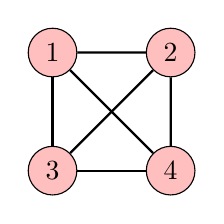
\begin{tikzpicture}[node distance=2cm, scale=1.5]

\node[draw, shape=circle, fill=pink] (1) at (0,1 ) {1};
\node[draw, shape=circle, fill=pink] (2)  at (1,1) {2};
\node[draw, shape=circle, fill=pink] (3)  at (0,0) {3};
\node[draw, shape=circle, fill=pink] (4)  at (1,0){4};
 
\draw[-, thick] (1) to (2);
\draw[-, thick] (1) to (3);
\draw[-, thick] (1) to (4);
\draw[-, thick] (2) to (3);
\draw[-, thick] (3) to (4);
\draw[-, thick] (2) to (4);
\end{tikzpicture}
\end{center}
 
\begin{center}
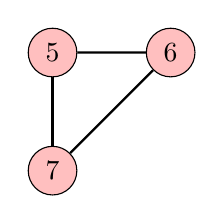
\begin{tikzpicture}[node distance=2cm, scale=1.5]

\node[draw, shape=circle, fill=pink] (5) at (0,1 ) {5};
\node[draw, shape=circle, fill=pink] (6)  at (1,1) {6};
\node[draw, shape=circle, fill=pink] (7)  at (0,0) {7};

 
\draw[-, thick] (5) to (6);
\draw[-, thick] (5) to (7);
\draw[-, thick] (6) to (7);
\end{tikzpicture}
\end{center}

\begin{center}
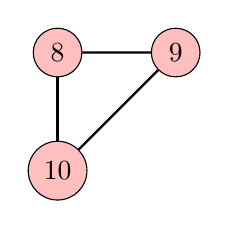
\begin{tikzpicture}[node distance=2cm, scale=1.5]

\node[draw, shape=circle, fill=pink] (8) at (0,1 ) {8};
\node[draw, shape=circle, fill=pink] (9)  at (1,1) {9};
\node[draw, shape=circle, fill=pink] (10)  at (0,0) {10};

 
\draw[-, thick] (8) to (9);
\draw[-, thick] (8) to (10);
\draw[-, thick] (9) to (10);
\end{tikzpicture}
\end{center}

\begin{center}
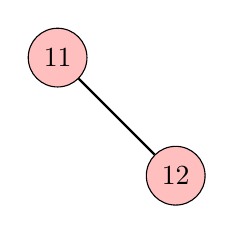
\begin{tikzpicture}[node distance=2cm, scale=1.5]

\node[draw, shape=circle, fill=pink] (11) at (0,1 ) {11};
\node[draw, shape=circle, fill=pink] (12)  at (1,0){12};
 
\draw[-, thick] (11) to (12);

\end{tikzpicture}
\end{center}
 



	\item[\textbf{b.}] \textbf{(7 points)} 

For every node $ i\in V$ with degree k, the clique generated $C_i$ contains the node $i$ iteself plus all its neighbors, and they are pairwise connected. Therefore, there are $k+1$ nodes in the clique $C_i$, and every node has degree of $k$. Run through all nodes in $G$, we get the degree distribution of $\widetilde{G}$:

$$ \widetilde{p} (x=k) = \frac{Number of nodes with degree k}{Total number of nodes in \widetilde{G}} $$ 
$$=\frac{|V| \times p(x=k) \times (k+1)}{\sum_{k=0}^\bigtriangleup |V| \times p(x=k) \times (k+1)}$$
$$=\frac{p(x=k) \times (k+1)}{\sum_{k=0}^\bigtriangleup  p(x=k) \times (k+1)}$$

	\item[\textbf{c.}] \textbf{(8 points)}  

Suppose that $p$ has the power-law property until $\bigtriangleup$, that is:
$$ \frac{p(k\prime)}{p(k)} \ge  (\frac{k\prime}{k})^{-\beta}$$ 
$$ \Rightarrow \frac{\widetilde{p}(k\prime)}{\widetilde{p}(k)} = \frac{\widetilde{p}(k\prime) (k\prime+1)}{\widetilde{p}(k) (k+1)} $$
$$ \ge (\frac{k\prime}{k})^{-\beta} \frac{k\prime+1}{k+1} \ge (\frac{k\prime}{k})^{-(\beta+1)}$$ 

The last inequality is due to the fact that $ (\frac{k\prime+1}{k+1})^{-1} \ge (\frac{k\prime}{k})^{-1}$.

Therefore, $\widetilde{p}$ has the power-law property until $\bigtriangleup$ as well with constant $\beta+1$. 


	\item[\textbf{d.}] \textbf{(7 points)} 
In networks whose degree distributions have the power law property, the "strong form" of the friendship paradox does not necessarily hold true. We have seen above that the graph $\widetilde{G}$ has a power law property, but for each node $i$ in the network, the avergae degree of $i's$ neighbors is equal to $i's$ own degree, since all i's neighbors have the same degree as $i$ does. This statement is subtly different from what we talked about in class. in the sense that, the "friendship paradox" focuses on the average degree of all nodes and avergae degree of all the neighbors, over all nodes in the network; while here we are talking about a specific node $i$, not average across the network. 

 
\end{enumerate}

\paragraph{5. Coding: Fitting Power-Laws (30 points).}


\begin{itemize}
	\item[\textbf{a.}] \textbf{(5 points)} 

The degree distribution of network1 and network2, respectively.

	\includegraphics[width=6in]{Q5a.png}

	\item[\textbf{b.}] \textbf{(5 points)} 

The log-log plot of degree distribution of network1 and network2, respectively.

	\includegraphics[width=6in]{Q5b.png}

	\item[\textbf{c.}] \textbf{(7 points)} 
 
Network 1 has $\alpha$ estimated using OLS: 1.9741. 

Network 2 has $\alpha$ estimated using OLS: 1.8204.

	\item[\textbf{d.}] \textbf{(10 points)} 
 
Network 1 has $\alpha$ estimated using Maximum Likelihood: 1.7422.

Network 2 has $\alpha$ estimated using Maximum Likelihood: 2.7299.

	\item[\textbf{e.}] \textbf{(3 points)}

For Network1, using OLS, degree distribution and log-log plot of degree distribution, respectively. 

	\includegraphics[width=6in]{Q5e1.png}

For Network1, using MLE, degree distribution and log-log plot of degree distribution, respectively. 

	\includegraphics[width=6in]{Q5e2.png}

For Network2, using OLS, degree distribution and log-log plot of degree distribution, respectively. 

	\includegraphics[width=6in]{Q5e3.png}

For Network2, using MLE, degree distribution and log-log plot of degree distribution, respectively. 

	\includegraphics[width=6in]{Q5e4.png}


The Ordinary Least Square approach has one major drawback, that is: we try to fit a straight line with 2 degrees of freedom (the intercept and the slope), assuming that the estimated slope approximates the $\alpha$ of our power-law distributino, while allowing the intercept estimated separately to minimize the sum of the squared residuals. However, if the data follows a power-law distribution as we derived in class, then the log-log plot's intercept is determined by the $\alpha$ as well, in other words, the intercept and the slope should not be estimated separately, as what OLS does. We actually only have one parameter alpha to estimate, not two parameters, therefore, technically, it does not satisfy ordinary least square approach assumption. Although convenient to estimate via OLS, the estimated $\alpha$ is not accurate.

The maximum likelihood is more appropriate, in the sense that, given the assumtption that the data follows a power-law distribution, we don't put additional unrealistic assumptions into the estimation process. We simply ask the parameter $\alpha$ for which the observed data is most likely to been drawn from the distribution. Therefore, we should estimate via ML, rather than OLS approach.

\end{itemize}




\end{document}
